% Forløbig resultater
% Opsætning
% Fuel
% Afstand
% Fremtidige tests/arbejde
% Konklusion


\section{Evaluation}
\begin{frame}{Test Setup}



\begin{columns}
	\begin{column}{0.7\textwidth}
		\begin{itemize}
		\item SUMO- Simulation of Urban MObility\\
		\item Real world road network\\
		\item Real world Traffic light phases\\
		\item Real world OD matrix\\
		\end{itemize}
	\end{column}

	\begin{column}{0.3\textwidth}
		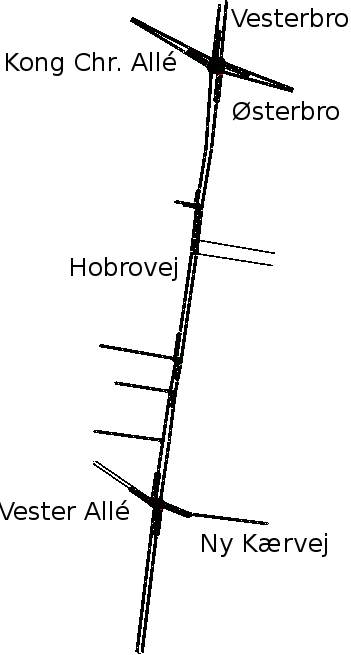
\includegraphics[width=0.8\textwidth]{images/Hobrovej.png}
	\end{column}
\end{columns}
\end{frame}

\begin{frame}{SUMO presentation}
\end{frame}

\begin{frame}{Fuelsaving}
	\begin{figure}
	\begin{tikzpicture}[scale=0.6]
	\begin{axis}[xlabel=Routes,xticklabel=\empty,ylabel=Fuel consumption,bar width=1pt,]
	\addplot[ybar, blue] table[x=Route,y=Fuel] {TestResults/0/avg.dat};
	\addplot[ybar, red] table[x=Route,y=Fuel] {TestResults/100/avg.dat};
	\draw[thick, red] (axis cs:0,138) -- (axis cs:109,138);
	\draw[thick, blue] (axis cs:0,162) -- (axis cs:109,162);
	\end{axis}
	\end{tikzpicture}
	\caption{Average fuel consumption with (red) and without \tech (blue)}\label{tik:fuel:avg}
	\end{figure}
\end{frame}


\begin{frame}{Distance}



\begin{columns}
	\begin{column}{0.5\textwidth}
	
\begin{figure}
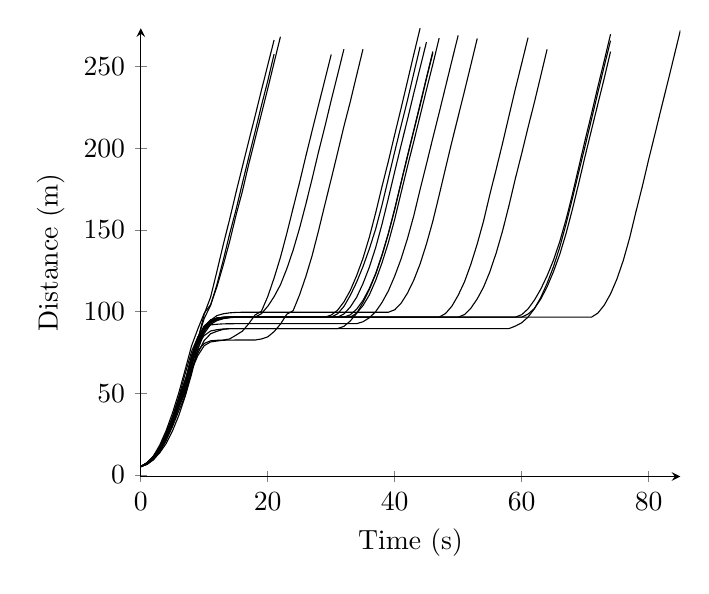
\begin{tikzpicture}
\begin{axis}[
legend style={anchor=west},
axis x line=bottom,
axis y line=left,
ymin=-1,
xlabel=Time (s),
ylabel=Distance (m),
]
\addplot[] coordinates {
(0, 5.1)
(1, 6.97200775137)
(2, 10.4286696057)
(3, 15.7069381488)
(4, 22.7175004247)
(5, 31.099567828)
(6, 41.7303372124)
(7, 51.6896584418)
(8, 66.8331596565)
(9, 79.9056524603)
(10, 88.1768936186)
(11, 92.9978698607)
(12, 94.9512971866)
(13, 96.3185424789)
(14, 96.5058699285)
(15, 96.5584462975)
(16, 96.5794598684)
(17, 96.5889410169)
(18, 96.5889410169)
(19, 96.5889410169)
(20, 96.5889410169)
(21, 96.5889410169)
(22, 96.5889410169)
(23, 96.5889410169)
(24, 96.5889410169)
(25, 96.5889410169)
(26, 96.5889410169)
(27, 96.5889410169)
(28, 96.5889410169)
(29, 96.5889410169)
(30, 96.5889410169)
(31, 96.5889410169)
(32, 98.5632673245)
(33, 102.768358719)
(34, 108.708036702)
(35, 117.082232403)
(36, 127.119294417)
(37, 139.147189714)
(38, 153.461905452)
(39, 169.322487058)
(40, 185.675380058)
(41, 201.755208248)
(42, 217.419099094)
(43, 233.588234424)
(44, 249.294751932)
(45, 264.937595934)
};
\addplot[] coordinates {
(0, 5.1)
(1, 7.4060649191)
(2, 11.3129873733)
(3, 16.6917972149)
(4, 23.8763369663)
(5, 32.8843378833)
(6, 44.1991027543)
(7, 53.9290850188)
(8, 68.5859185959)
(9, 81.1622642551)
(10, 89.9189182174)
(11, 94.1029290622)
(12, 95.5712814771)
(13, 96.3567333977)
(14, 96.5002379197)
(15, 96.5512906596)
(16, 96.5888029021)
(17, 96.5888029021)
(18, 96.5888029021)
(19, 96.5888029021)
(20, 96.5888029021)
(21, 96.5888029021)
(22, 96.5888029021)
(23, 96.5888029021)
(24, 96.5888029021)
(25, 96.5888029021)
(26, 96.5888029021)
(27, 96.5888029021)
(28, 96.5888029021)
(29, 96.5888029021)
(30, 96.5888029021)
(31, 96.5888029021)
(32, 96.5888029021)
(33, 96.5888029021)
(34, 96.5888029021)
(35, 96.5888029021)
(36, 96.5888029021)
(37, 96.5888029021)
(38, 96.5888029021)
(39, 96.5888029021)
(40, 96.5888029021)
(41, 96.5888029021)
(42, 96.5888029021)
(43, 96.5888029021)
(44, 96.5888029021)
(45, 96.5888029021)
(46, 96.5888029021)
(47, 96.5888029021)
(48, 96.5888029021)
(49, 96.5888029021)
(50, 96.5888029021)
(51, 96.5888029021)
(52, 96.5888029021)
(53, 96.5888029021)
(54, 96.5888029021)
(55, 96.5888029021)
(56, 96.5888029021)
(57, 96.5888029021)
(58, 96.5888029021)
(59, 96.5888029021)
(60, 98.0916425418)
(61, 101.622408149)
(62, 106.973976088)
(63, 113.673744847)
(64, 121.837226247)
(65, 131.406755344)
(66, 142.86238716)
(67, 156.48929864)
(68, 171.992202967)
(69, 188.551889599)
(70, 205.129560577)
(71, 221.108945946)
(72, 237.675963341)
(73, 253.464916314)
(74, 269.78566888)
};
\addplot[] coordinates {
(0, 5.1)
(1, 6.94645065136)
(2, 10.2182143818)
(3, 15.450534422)
(4, 22.9516846069)
(5, 32.4742679483)
(6, 44.2010389526)
(7, 54.9907672875)
(8, 70.4218299565)
(9, 82.2000333449)
(10, 89.8085650479)
(11, 94.032886936)
(12, 95.3128484207)
(13, 95.915269957)
(14, 96.3751516442)
(15, 96.5617414633)
(16, 96.5794471041)
(17, 96.585542104)
(18, 96.585542104)
(19, 96.585542104)
(20, 96.585542104)
(21, 96.585542104)
(22, 96.585542104)
(23, 96.585542104)
(24, 96.585542104)
(25, 96.585542104)
(26, 96.585542104)
(27, 96.585542104)
(28, 96.585542104)
(29, 96.585542104)
(30, 96.585542104)
(31, 96.585542104)
(32, 96.585542104)
(33, 98.0156274022)
(34, 101.447440714)
(35, 106.801021541)
(36, 114.130274172)
(37, 123.198194746)
(38, 134.394764779)
(39, 147.679888574)
(40, 163.024991707)
(41, 178.962784633)
(42, 194.722641625)
(43, 210.646967073)
(44, 226.230740394)
(45, 242.616777347)
(46, 258.240138956)
};
\addplot[] coordinates {
(0, 5.1)
(1, 6.54597713341)
(2, 9.27388870585)
(3, 14.0656536008)
(4, 21.0818730794)
(5, 30.3446806859)
(6, 41.8111165283)
(7, 51.7211102683)
(8, 66.9564409532)
(9, 82.9024469562)
(10, 98.4890786174)
(11, 108.856734219)
(12, 124.714248183)
(13, 141.079552088)
(14, 156.535532258)
(15, 172.880524159)
(16, 188.585259091)
(17, 204.225425949)
(18, 219.597653978)
(19, 235.412150904)
(20, 250.809611203)
(21, 266.257557063)
};
\addplot[] coordinates {
(0, 5.1)
(1, 6.88304061381)
(2, 10.0573408472)
(3, 15.468693347)
(4, 22.7800063546)
(5, 31.4310592686)
(6, 41.5846322048)
(7, 50.1726741158)
(8, 64.1418514701)
(9, 73.109531037)
(10, 79.149980641)
(11, 81.4046054309)
(12, 81.9697957356)
(13, 82.4525739492)
(14, 82.5366180613)
(15, 82.5710512764)
(16, 82.5710512764)
(17, 82.5710512764)
(18, 82.5710512764)
(19, 83.225611438)
(20, 84.5055901812)
(21, 87.7109927496)
(22, 92.2832884322)
(23, 98.3656813858)
(24, 100.527530704)
(25, 110.102228261)
(26, 121.433593438)
(27, 134.367055417)
(28, 149.482795007)
(29, 165.494087865)
(30, 181.16423177)
(31, 197.167989456)
(32, 213.384133244)
(33, 228.43614776)
(34, 244.616915189)
(35, 260.608799622)
};
\addplot[] coordinates {
(0, 5.1)
(1, 7.325701774)
(2, 11.046752624)
(3, 17.2405710478)
(4, 25.2693241668)
(5, 35.3554105481)
(6, 47.8008066975)
(7, 61.9624091582)
(8, 75.5530629442)
(9, 84.4225091474)
(10, 89.0713791589)
(11, 91.8399807842)
(12, 92.2410448865)
(13, 92.4741940102)
(14, 92.5731221811)
(15, 92.5803398683)
(16, 92.5803398683)
(17, 92.5803398683)
(18, 92.5803398683)
(19, 92.5803398683)
(20, 92.5803398683)
(21, 92.5803398683)
(22, 92.5803398683)
(23, 92.5803398683)
(24, 92.5803398683)
(25, 92.5803398683)
(26, 92.5803398683)
(27, 92.5803398683)
(28, 92.5803398683)
(29, 92.5803398683)
(30, 92.5803398683)
(31, 92.5803398683)
(32, 92.5803398683)
(33, 92.5803398683)
(34, 92.5803398683)
(35, 93.7533093719)
(36, 96.1924873408)
(37, 99.9292764305)
(38, 105.565945877)
(39, 112.640426429)
(40, 121.719081133)
(41, 132.196530131)
(42, 144.556927861)
(43, 158.589659642)
(44, 174.755868109)
(45, 190.280109575)
(46, 206.171287897)
(47, 221.700199679)
(48, 237.554659528)
(49, 253.440683484)
(50, 269.131994829)
};
\addplot[] coordinates {
(0, 5.1)
(1, 6.56262268538)
(2, 9.44773200051)
(3, 13.602592154)
(4, 19.2104367254)
(5, 26.9377255012)
(6, 36.4670034807)
(7, 48.1178167635)
(8, 61.6697898104)
(9, 77.0941921456)
(10, 87.8822723794)
(11, 94.6289486843)
(12, 97.5571131021)
(13, 98.6543127741)
(14, 99.2218635499)
(15, 99.4769168347)
(16, 99.5782242958)
(17, 99.5849358413)
(18, 99.5849358413)
(19, 99.5849358413)
(20, 99.5849358413)
(21, 99.5849358413)
(22, 99.5849358413)
(23, 99.5849358413)
(24, 99.5849358413)
(25, 99.5849358413)
(26, 99.5849358413)
(27, 99.5849358413)
(28, 99.5849358413)
(29, 99.5849358413)
(30, 99.5849358413)
(31, 99.5849358413)
(32, 99.5849358413)
(33, 99.5849358413)
(34, 99.5849358413)
(35, 99.5849358413)
(36, 99.5849358413)
(37, 99.5849358413)
(38, 99.5849358413)
(39, 99.5849358413)
(40, 101.094643165)
(41, 105.077689309)
(42, 111.223923354)
(43, 119.199474771)
(44, 129.139835145)
(45, 141.354078079)
(46, 155.256285361)
(47, 171.213161228)
(48, 187.642072894)
(49, 203.867728038)
(50, 219.437997898)
(51, 235.125112176)
(52, 251.068242565)
(53, 267.18216759)
};
\addplot[] coordinates {
(0, 5.1)
(1, 7.28192367436)
(2, 11.0529181573)
(3, 17.2121714651)
(4, 25.4973333395)
(5, 35.0742356507)
(6, 46.6258126921)
(7, 57.3508743576)
(8, 72.9563748666)
(9, 84.3224022542)
(10, 90.8829136561)
(11, 94.3649733027)
(12, 95.9161351033)
(13, 96.5016918189)
(14, 96.5813991727)
(15, 96.5813991727)
(16, 96.5813991727)
(17, 96.5813991727)
(18, 96.5813991727)
(19, 96.5813991727)
(20, 96.5813991727)
(21, 96.5813991727)
(22, 96.5813991727)
(23, 96.5813991727)
(24, 96.5813991727)
(25, 96.5813991727)
(26, 96.5813991727)
(27, 96.5813991727)
(28, 96.5813991727)
(29, 96.5813991727)
(30, 96.5813991727)
(31, 98.6438989858)
(32, 103.105980696)
(33, 109.89415601)
(34, 117.995718575)
(35, 127.514128662)
(36, 138.297742152)
(37, 150.540488768)
(38, 165.178384995)
(39, 181.512399256)
(40, 197.85527332)
(41, 213.720082121)
(42, 229.223278363)
(43, 245.79681041)
(44, 262.117374268)
};
\addplot[] coordinates {
(0, 5.1)
(1, 7.03005183217)
(2, 11.2426145173)
(3, 17.152889397)
(4, 25.3541977243)
(5, 35.4259031454)
(6, 47.4216952704)
(7, 58.3965536525)
(8, 69.291233774)
(9, 76.2606868028)
(10, 80.4887391466)
(11, 82.1029529803)
(12, 82.4152451948)
(13, 82.5409377112)
(14, 83.241416191)
(15, 85.5473848812)
(16, 87.9695838735)
(17, 92.515549333)
(18, 97.9200445326)
(19, 100.142145493)
(20, 109.149278393)
(21, 120.509098434)
(22, 133.178658896)
(23, 147.796031914)
(24, 163.41414254)
(25, 178.815522162)
(26, 195.106608252)
(27, 210.864119522)
(28, 226.412805784)
(29, 241.848324393)
(30, 257.423889648)
};
\addplot[] coordinates {
(0, 5.1)
(1, 7.2400267677)
(2, 11.0705113627)
(3, 16.3230058246)
(4, 23.0933234687)
(5, 31.7622075818)
(6, 42.3026258044)
(7, 51.1432181588)
(8, 64.5993130931)
(9, 74.6137445512)
(10, 82.3076412407)
(11, 86.3905616125)
(12, 87.9442723068)
(13, 89.1234722534)
(14, 89.5489040344)
(15, 89.5686457182)
(16, 89.5782162288)
(17, 89.5782162288)
(18, 89.5782162288)
(19, 89.5782162288)
(20, 89.5782162288)
(21, 89.5782162288)
(22, 89.5782162288)
(23, 89.5782162288)
(24, 89.5782162288)
(25, 89.5782162288)
(26, 89.5782162288)
(27, 89.5782162288)
(28, 89.5782162288)
(29, 89.5782162288)
(30, 89.5782162288)
(31, 89.5782162288)
(32, 89.5782162288)
(33, 89.5782162288)
(34, 89.5782162288)
(35, 89.5782162288)
(36, 89.5782162288)
(37, 89.5782162288)
(38, 89.5782162288)
(39, 89.5782162288)
(40, 89.5782162288)
(41, 89.5782162288)
(42, 89.5782162288)
(43, 89.5782162288)
(44, 89.5782162288)
(45, 89.5782162288)
(46, 89.5782162288)
(47, 89.5782162288)
(48, 89.5782162288)
(49, 89.5782162288)
(50, 89.5782162288)
(51, 89.5782162288)
(52, 89.5782162288)
(53, 89.5782162288)
(54, 89.5782162288)
(55, 89.5782162288)
(56, 89.5782162288)
(57, 89.5782162288)
(58, 89.5782162288)
(59, 91.0991337251)
(60, 93.1387545872)
(61, 96.6200167714)
(62, 101.685891673)
(63, 108.555766861)
(64, 117.278141506)
(65, 127.362694138)
(66, 139.423020563)
(67, 153.769296688)
(68, 169.388346552)
(69, 185.575387923)
(70, 201.504028464)
(71, 217.748931785)
(72, 234.088769022)
(73, 250.178094333)
(74, 265.838515084)
};
\addplot[] coordinates {
(0, 5.1)
(1, 7.31061273856)
(2, 11.1963455483)
(3, 16.5901446184)
(4, 24.400431794)
(5, 34.1722540964)
(6, 45.3975576671)
(7, 55.424990925)
(8, 70.7089272369)
(9, 83.3138426886)
(10, 90.3305852703)
(11, 94.1248183611)
(12, 96.1914937187)
(13, 96.4518083621)
(14, 96.5351778375)
(15, 96.586098631)
(16, 96.586098631)
(17, 96.586098631)
(18, 96.586098631)
(19, 96.586098631)
(20, 96.586098631)
(21, 96.586098631)
(22, 96.586098631)
(23, 96.586098631)
(24, 96.586098631)
(25, 96.586098631)
(26, 96.586098631)
(27, 96.586098631)
(28, 96.586098631)
(29, 96.586098631)
(30, 96.586098631)
(31, 96.586098631)
(32, 96.586098631)
(33, 96.586098631)
(34, 96.586098631)
(35, 96.586098631)
(36, 96.586098631)
(37, 96.586098631)
(38, 96.586098631)
(39, 96.586098631)
(40, 96.586098631)
(41, 96.586098631)
(42, 96.586098631)
(43, 96.586098631)
(44, 96.586098631)
(45, 96.586098631)
(46, 96.586098631)
(47, 96.586098631)
(48, 96.586098631)
(49, 96.586098631)
(50, 96.586098631)
(51, 96.586098631)
(52, 96.586098631)
(53, 96.586098631)
(54, 96.586098631)
(55, 96.586098631)
(56, 96.586098631)
(57, 96.586098631)
(58, 96.586098631)
(59, 96.586098631)
(60, 96.586098631)
(61, 96.586098631)
(62, 96.586098631)
(63, 96.586098631)
(64, 96.586098631)
(65, 96.586098631)
(66, 96.586098631)
(67, 96.586098631)
(68, 96.586098631)
(69, 96.586098631)
(70, 96.586098631)
(71, 96.586098631)
(72, 99.054667082)
(73, 103.889378033)
(74, 110.826646527)
(75, 119.893969965)
(76, 131.22934428)
(77, 144.99558847)
(78, 161.143299092)
(79, 176.54934854)
(80, 193.081544329)
(81, 208.74899718)
(82, 224.713817209)
(83, 240.28224262)
(84, 256.209023282)
(85, 272.201756898)
};
\addplot[] coordinates {
(0, 5.1)
(1, 7.2008604957)
(2, 10.917367672)
(3, 16.2979551354)
(4, 23.1595678609)
(5, 32.0801552079)
(6, 42.7598994186)
(7, 52.3612871228)
(8, 66.2952646073)
(9, 79.5642767314)
(10, 87.971000528)
(11, 93.6298560686)
(12, 94.8721496277)
(13, 95.8345138835)
(14, 96.2760208428)
(15, 96.5247971594)
(16, 96.5795201214)
(17, 96.5855254155)
(18, 96.5855254155)
(19, 96.5855254155)
(20, 96.5855254155)
(21, 96.5855254155)
(22, 96.5855254155)
(23, 96.5855254155)
(24, 96.5855254155)
(25, 96.5855254155)
(26, 96.5855254155)
(27, 96.5855254155)
(28, 96.5855254155)
(29, 96.5855254155)
(30, 96.5855254155)
(31, 96.5855254155)
(32, 96.5855254155)
(33, 96.5855254155)
(34, 99.0098235259)
(35, 103.630174324)
(36, 110.144796045)
(37, 119.050709831)
(38, 129.846763955)
(39, 142.172508366)
(40, 156.515240202)
(41, 172.653680374)
(42, 188.649494544)
(43, 204.085421624)
(44, 219.850594625)
(45, 235.783322081)
(46, 251.23893284)
(47, 267.417199906)
};
\addplot[] coordinates {
(0, 5.1)
(1, 7.57943529073)
(2, 11.4659328129)
(3, 16.9589783521)
(4, 24.3790610858)
(5, 33.6792784236)
(6, 45.0260407392)
(7, 55.3340978697)
(8, 70.2082791866)
(9, 83.4593937671)
(10, 95.8438762658)
(11, 103.769747395)
(12, 116.622960042)
(13, 131.564876423)
(14, 147.572884327)
(15, 162.29541423)
(16, 178.476476014)
(17, 194.370876865)
(18, 209.929996107)
(19, 226.012645078)
(20, 241.171079717)
(21, 257.581800524)
};
\addplot[] coordinates {
(0, 5.1)
(1, 6.81952185017)
(2, 10.8366611707)
(3, 16.5942785868)
(4, 24.2584390475)
(5, 34.3133574173)
(6, 45.9922180612)
(7, 56.8632856137)
(8, 72.2598634504)
(9, 83.7100706393)
(10, 91.2782193337)
(11, 94.0749037828)
(12, 95.7061519849)
(13, 96.3295878531)
(14, 96.4951264217)
(15, 96.5676944692)
(16, 96.5885090711)
(17, 96.5885090711)
(18, 96.5885090711)
(19, 96.5885090711)
(20, 96.5885090711)
(21, 96.5885090711)
(22, 96.5885090711)
(23, 96.5885090711)
(24, 96.5885090711)
(25, 96.5885090711)
(26, 96.5885090711)
(27, 96.5885090711)
(28, 96.5885090711)
(29, 96.5885090711)
(30, 97.8490418053)
(31, 100.834091216)
(32, 105.912841418)
(33, 112.911745068)
(34, 121.976276187)
(35, 132.576443152)
(36, 145.46728752)
(37, 160.408922368)
(38, 176.583957785)
(39, 191.993400693)
(40, 208.38645069)
(41, 224.406307749)
(42, 240.842011648)
(43, 257.39074018)
(44, 273.471539844)
};
\addplot[] coordinates {
(0, 5.1)
(1, 6.49724314533)
(2, 9.50720913932)
(3, 14.7385154364)
(4, 21.4080015418)
(5, 29.5976414606)
(6, 39.3666279766)
(7, 48.5930163263)
(8, 63.3068912497)
(9, 77.3631411265)
(10, 86.5849520359)
(11, 92.1493112905)
(12, 94.4683727312)
(13, 95.6350051243)
(14, 96.3861247191)
(15, 96.5677289902)
(16, 96.5821547801)
(17, 96.5821547801)
(18, 96.5821547801)
(19, 96.5821547801)
(20, 96.5821547801)
(21, 96.5821547801)
(22, 96.5821547801)
(23, 96.5821547801)
(24, 96.5821547801)
(25, 96.5821547801)
(26, 96.5821547801)
(27, 96.5821547801)
(28, 96.5821547801)
(29, 96.5821547801)
(30, 96.5821547801)
(31, 96.5821547801)
(32, 96.5821547801)
(33, 96.5821547801)
(34, 96.5821547801)
(35, 96.5821547801)
(36, 96.5821547801)
(37, 96.5821547801)
(38, 96.5821547801)
(39, 96.5821547801)
(40, 96.5821547801)
(41, 96.5821547801)
(42, 96.5821547801)
(43, 96.5821547801)
(44, 96.5821547801)
(45, 96.5821547801)
(46, 96.5821547801)
(47, 96.5821547801)
(48, 96.5821547801)
(49, 96.5821547801)
(50, 96.5821547801)
(51, 96.5821547801)
(52, 96.5821547801)
(53, 96.5821547801)
(54, 96.5821547801)
(55, 96.5821547801)
(56, 96.5821547801)
(57, 96.5821547801)
(58, 96.5821547801)
(59, 96.5821547801)
(60, 96.5821547801)
(61, 98.4504914465)
(62, 101.8814718)
(63, 107.616276954)
(64, 115.121298266)
(65, 124.36453591)
(66, 135.007570993)
(67, 147.911858759)
(68, 162.716297589)
(69, 178.73822204)
(70, 195.278139504)
(71, 211.217566912)
(72, 227.076517402)
(73, 242.76328689)
(74, 259.175706924)
};
\addplot[] coordinates {
(0, 5.1)
(1, 6.96085600522)
(2, 10.6836619282)
(3, 16.8386651941)
(4, 25.2060684753)
(5, 35.0426150229)
(6, 46.5006141532)
(7, 56.8620938922)
(8, 72.6008244491)
(9, 84.3963668478)
(10, 90.9988697718)
(11, 94.9807510432)
(12, 95.8665820037)
(13, 96.4396761263)
(14, 96.5217914901)
(15, 96.5870731209)
(16, 96.5870731209)
(17, 96.5870731209)
(18, 96.5870731209)
(19, 96.5870731209)
(20, 96.5870731209)
(21, 96.5870731209)
(22, 96.5870731209)
(23, 96.5870731209)
(24, 96.5870731209)
(25, 96.5870731209)
(26, 96.5870731209)
(27, 96.5870731209)
(28, 96.5870731209)
(29, 96.5870731209)
(30, 96.5870731209)
(31, 96.5870731209)
(32, 96.5870731209)
(33, 96.5870731209)
(34, 96.5870731209)
(35, 96.5870731209)
(36, 96.5870731209)
(37, 96.5870731209)
(38, 96.5870731209)
(39, 96.5870731209)
(40, 96.5870731209)
(41, 96.5870731209)
(42, 96.5870731209)
(43, 96.5870731209)
(44, 96.5870731209)
(45, 96.5870731209)
(46, 96.5870731209)
(47, 96.5870731209)
(48, 98.7967090267)
(49, 103.266753288)
(50, 109.971030357)
(51, 118.274927208)
(52, 128.97554941)
(53, 141.422022338)
(54, 155.463136635)
(55, 171.914602301)
(56, 187.321373008)
(57, 203.20555435)
(58, 219.778825189)
(59, 236.276900988)
(60, 251.834816372)
(61, 267.686416971)
};
\addplot[] coordinates {
(0, 5.1)
(1, 7.35183463976)
(2, 11.181624715)
(3, 16.649240243)
(4, 24.4811478463)
(5, 34.6150674964)
(6, 46.4014904814)
(7, 56.658120018)
(8, 70.4703530553)
(9, 80.3603185873)
(10, 85.3057858088)
(11, 88.1185451021)
(12, 88.9039391901)
(13, 89.3537115135)
(14, 89.5612616919)
(15, 89.5806505586)
(16, 89.5806505586)
(17, 89.5806505586)
(18, 89.5806505586)
(19, 89.5806505586)
(20, 89.5806505586)
(21, 89.5806505586)
(22, 89.5806505586)
(23, 89.5806505586)
(24, 89.5806505586)
(25, 89.5806505586)
(26, 89.5806505586)
(27, 89.5806505586)
(28, 89.5806505586)
(29, 89.5806505586)
(30, 89.5806505586)
(31, 89.5806505586)
(32, 90.9584791701)
(33, 94.2269543632)
(34, 98.9008467537)
(35, 105.54023449)
(36, 113.466868298)
(37, 122.956637284)
(38, 134.697687118)
(39, 147.84736334)
(40, 162.384078344)
(41, 178.878068152)
(42, 195.262402742)
(43, 210.955681081)
(44, 227.070610659)
(45, 243.130219717)
(46, 259.203657599)
};
\addplot[] coordinates {
(0, 5.1)
(1, 6.87223047038)
(2, 10.8200329183)
(3, 16.2783040466)
(4, 23.3135765866)
(5, 32.6292317418)
(6, 43.4239200531)
(7, 53.1003742712)
(8, 67.9245255941)
(9, 80.8185234645)
(10, 89.0383235593)
(11, 94.1657930139)
(12, 95.8804524771)
(13, 96.4579836915)
(14, 96.5463158631)
(15, 96.5731202088)
(16, 96.584942047)
(17, 96.584942047)
(18, 96.584942047)
(19, 96.584942047)
(20, 96.584942047)
(21, 96.584942047)
(22, 96.584942047)
(23, 96.584942047)
(24, 96.584942047)
(25, 96.584942047)
(26, 96.584942047)
(27, 96.584942047)
(28, 96.584942047)
(29, 96.584942047)
(30, 96.584942047)
(31, 96.584942047)
(32, 96.584942047)
(33, 96.584942047)
(34, 96.584942047)
(35, 96.584942047)
(36, 96.584942047)
(37, 96.584942047)
(38, 96.584942047)
(39, 96.584942047)
(40, 96.584942047)
(41, 96.584942047)
(42, 96.584942047)
(43, 96.584942047)
(44, 96.584942047)
(45, 96.584942047)
(46, 96.584942047)
(47, 96.584942047)
(48, 96.584942047)
(49, 96.584942047)
(50, 96.584942047)
(51, 98.1789396445)
(52, 102.081165593)
(53, 107.75970184)
(54, 115.008479895)
(55, 124.451498901)
(56, 136.061906841)
(57, 149.527504421)
(58, 164.888024821)
(59, 181.360084078)
(60, 196.716365061)
(61, 212.681266905)
(62, 228.064266355)
(63, 244.195990011)
(64, 260.510722638)
};
\addplot[] coordinates {
(0, 5.1)
(1, 7.09090068956)
(2, 11.5778575712)
(3, 18.3541636672)
(4, 27.1478501756)
(5, 37.9636761327)
(6, 50.4130363405)
(7, 64.4640885831)
(8, 79.0538572907)
(9, 89.465255557)
(10, 99.0625037512)
(11, 104.161843115)
(12, 115.206689267)
(13, 128.557609273)
(14, 142.878757745)
(15, 158.935726384)
(16, 173.506423121)
(17, 190.088485233)
(18, 205.513343567)
(19, 220.952319013)
(20, 236.399577398)
(21, 252.405980221)
(22, 268.275035152)
};
\addplot[] coordinates {
(0, 5.1)
(1, 7.18780044602)
(2, 10.6284556738)
(3, 15.7732518849)
(4, 23.4053818313)
(5, 33.4100594001)
(6, 45.4521411237)
(7, 56.535312748)
(8, 71.8956960544)
(9, 83.3932370191)
(10, 90.1956726826)
(11, 93.6779453998)
(12, 95.9924541814)
(13, 96.4785709478)
(14, 96.5801640281)
(15, 96.5801640281)
(16, 96.5801640281)
(17, 96.5801640281)
(18, 96.5801640281)
(19, 98.6912794761)
(20, 103.214040946)
(21, 109.093501028)
(22, 116.385761794)
(23, 126.139132884)
(24, 137.597103612)
(25, 150.876296463)
(26, 165.711443331)
(27, 181.42850117)
(28, 197.765561776)
(29, 213.177666195)
(30, 229.407632512)
(31, 244.867679714)
(32, 260.651587677)
};

\end{axis}
\end{tikzpicture}
\label{tik:0:1_S, 1_S.-60, 2_V}
\caption{0 percent diving with GSC on route $1_S, 1_S.-60, 2_V$}
\end{figure}

	\end{column}

	\begin{column}{0.5\textwidth}
	
\begin{figure}
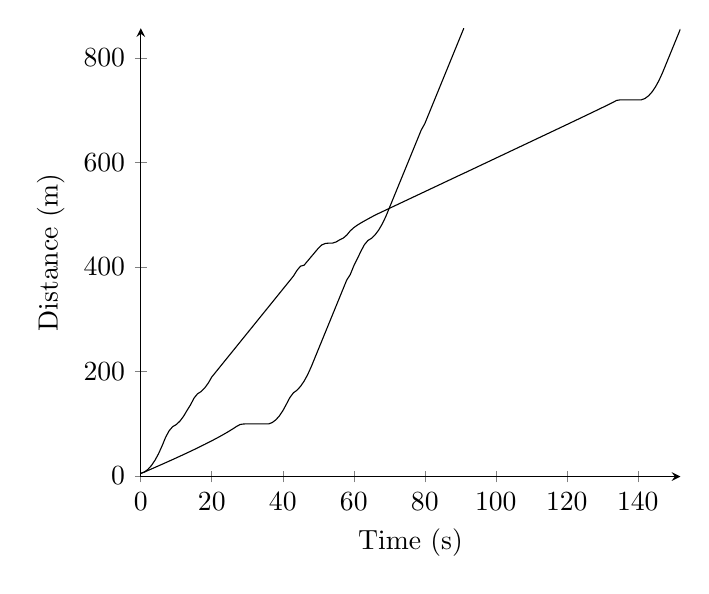
\begin{tikzpicture}
\begin{axis}[
legend style={anchor=west},
axis x line=bottom,
axis y line=left,
ymin=-1,
xlabel=Time (s),
ylabel=Distance (m),
]
\addplot[] coordinates {
(0, 5.1)
(1, 7.6)
(2, 10.551264739)
(3, 13.5148458518)
(4, 16.491720024)
(5, 19.4829705626)
(6, 22.4898024406)
(7, 25.5135599774)
(8, 28.555747716)
(9, 31.6180551961)
(10, 34.7023865031)
(11, 37.810895714)
(12, 40.9460296665)
(13, 44.1105798987)
(14, 47.3077461535)
(15, 50.5412145976)
(16, 53.8152549271)
(17, 57.1348419561)
(18, 60.5058092771)
(19, 63.9350454196)
(20, 67.4307470306)
(21, 71.0027496137)
(22, 74.6629653545)
(23, 78.4259712621)
(24, 82.309812202)
(25, 86.3371174595)
(26, 90.5366852977)
(27, 94.9457842613)
(28, 98.6044896023)
(29, 99.6320158223)
(30, 99.7193641886)
(31, 99.7193641886)
(32, 99.7193641886)
(33, 99.7193641886)
(34, 99.7193641886)
(35, 99.7193641886)
(36, 99.7193641886)
(37, 102.219364189)
(38, 107.219364189)
(39, 114.719364189)
(40, 124.719364189)
(41, 137.219364189)
(42, 150.125095958)
(43, 159.234657451)
(44, 164.142641251)
(45, 171.550625052)
(46, 181.458608852)
(47, 193.866592652)
(48, 208.774576453)
(49, 225.374576453)
(50, 241.974576453)
(51, 258.574576453)
(52, 275.174576453)
(53, 291.774576453)
(54, 308.374576453)
(55, 324.974576453)
(56, 341.574576453)
(57, 358.174576453)
(58, 374.774576453)
(59, 385.384576453)
(60, 401.984576453)
(61, 415.584576453)
(62, 429.92347141)
(63, 442.651450477)
(64, 450.734866052)
(65, 454.801722929)
(66, 461.368579805)
(67, 470.435436682)
(68, 482.002293558)
(69, 496.069150435)
(70, 512.636007311)
(71, 529.236007311)
(72, 545.836007311)
(73, 562.436007311)
(74, 578.936007311)
(75, 595.536007311)
(76, 612.136007311)
(77, 628.736007311)
(78, 645.336007311)
(79, 661.936007311)
(80, 674.076007311)
(81, 690.676007311)
(82, 707.276007311)
(83, 723.876007311)
(84, 740.476007311)
(85, 757.076007311)
(86, 773.676007311)
(87, 790.276007311)
(88, 806.876007311)
(89, 823.476007311)
(90, 840.076007311)
(91, 856.676007311)
};
\addplot[] coordinates {
(0, 5.1)
(1, 7.6)
(2, 12.6)
(3, 20.1)
(4, 30.1)
(5, 42.6)
(6, 57.6)
(7, 74.2)
(8, 86.6997297278)
(9, 94.5649106955)
(10, 98.4573862023)
(11, 104.849861709)
(12, 113.742337216)
(13, 125.134812723)
(14, 136.02728823)
(15, 149.039719459)
(16, 157.36882852)
(17, 161.634015209)
(18, 168.399201898)
(19, 177.664388587)
(20, 189.429575276)
(21, 197.822653454)
(22, 206.215777321)
(23, 214.6089514)
(24, 223.002180831)
(25, 231.39547148)
(26, 239.788830074)
(27, 248.182264361)
(28, 256.575783316)
(29, 264.969397389)
(30, 273.363118827)
(31, 281.756962071)
(32, 290.150944275)
(33, 298.545085976)
(34, 306.939411965)
(35, 315.333952455)
(36, 323.728744648)
(37, 332.123834879)
(38, 340.519281603)
(39, 348.915159643)
(40, 357.311566345)
(41, 365.708630755)
(42, 374.106527678)
(43, 382.505499944)
(44, 393.404472211)
(45, 401.495043603)
(46, 403.315921389)
(47, 411.406228382)
(48, 419.498021114)
(49, 427.592671136)
(50, 435.692811781)
(51, 442.135492037)
(52, 444.939362145)
(53, 445.562177829)
(54, 445.594416168)
(55, 447.718518537)
(56, 451.744076421)
(57, 455.010741568)
(58, 460.777406715)
(59, 468.983220762)
(60, 475.126173639)
(61, 479.98217806)
(62, 484.165440335)
(63, 488.045666837)
(64, 491.801513568)
(65, 495.508625682)
(66, 499.197053628)
(67, 502.398679294)
(68, 505.60038685)
(69, 508.802179833)
(70, 512.00406199)
(71, 515.206037288)
(72, 518.408109936)
(73, 521.610284397)
(74, 524.812565414)
(75, 528.014958028)
(76, 531.217467605)
(77, 534.420099859)
(78, 537.622860883)
(79, 540.825757181)
(80, 544.028795704)
(81, 547.231983886)
(82, 550.43532969)
(83, 553.638841654)
(84, 556.842528945)
(85, 560.046401418)
(86, 563.250469681)
(87, 566.454745168)
(88, 569.659240225)
(89, 572.863968196)
(90, 576.068943533)
(91, 579.17418191)
(92, 582.384466492)
(93, 585.594782946)
(94, 588.80513343)
(95, 592.015520299)
(96, 595.225946133)
(97, 598.436413761)
(98, 601.646926294)
(99, 604.857487159)
(100, 608.068100143)
(101, 611.278769439)
(102, 614.489499704)
(103, 617.700296122)
(104, 620.911164487)
(105, 624.122111289)
(106, 627.333143825)
(107, 630.54427033)
(108, 633.755500132)
(109, 636.966843838)
(110, 640.178313567)
(111, 643.389923225)
(112, 646.601688852)
(113, 649.81362905)
(114, 653.025765514)
(115, 656.238123711)
(116, 659.450733742)
(117, 662.663631452)
(118, 665.876859877)
(119, 669.090471166)
(120, 672.304426716)
(121, 675.540738148)
(122, 678.778922376)
(123, 682.019357719)
(124, 685.262533559)
(125, 688.509095201)
(126, 691.759912938)
(127, 695.016192554)
(128, 698.279660573)
(129, 701.552893549)
(130, 704.839949662)
(131, 708.147712295)
(132, 711.489214454)
(133, 714.894166483)
(134, 718.464164333)
(135, 719.59368241)
(136, 719.699074378)
(137, 719.699074378)
(138, 719.699074378)
(139, 719.699074378)
(140, 719.699074378)
(141, 719.699074378)
(142, 722.199074378)
(143, 727.199074378)
(144, 734.699074378)
(145, 744.699074378)
(146, 757.199074378)
(147, 772.199074378)
(148, 788.799074378)
(149, 805.399074378)
(150, 821.999074378)
(151, 838.599074378)
(152, 855.199074378)
};

\end{axis}
\end{tikzpicture}
\label{tik:distance:100:53}
\caption{100 percent diving with GSC on route $53$}
\end{figure}

	\end{column}
\end{columns}
\end{frame}
